% SCIENCE Visual Guide 2.0.1 + AI_SKILLS_R5; Akulin--Karlov batch v2.
% Graph traces are visibly heavier than axes. All labels use anchored positions.
\documentclass[border=5pt]{standalone}
\usepackage{fontspec,unicode-math}
\setmainfont{Noto Sans}
\setsansfont{Noto Sans}
\setmathfont{STIXTwoMath-Regular.otf}
\usepackage{tikz}
\usetikzlibrary{arrows.meta,calc,patterns,decorations.pathreplacing,intersections}
\definecolor{ScienceInk}{HTML}{000000}
\definecolor{ScienceCurve}{HTML}{000000}
\definecolor{ScienceAux}{HTML}{000000}
\definecolor{ScienceMuted}{HTML}{000000}
\tikzset{
  axis/.style={draw=ScienceInk,line width=0.75pt,-{Latex[length=2.2mm,width=1.35mm]}},
  axisplain/.style={draw=ScienceInk,line width=0.70pt},
  curve/.style={draw=ScienceCurve,line width=2.15pt,line cap=round,line join=round},
  curveb/.style={draw=ScienceAux,line width=1.95pt,dash pattern=on 6pt off 2.4pt,line cap=round,line join=round},
  curvedash/.style={draw=ScienceAux,line width=1.9pt,dash pattern=on 4pt off 3pt},
  optbeam/.style={draw=ScienceCurve,line width=1.75pt,-{Latex[length=2.2mm,width=1.3mm]}},
  optback/.style={draw=ScienceAux,line width=1.65pt,-{Latex[length=2mm,width=1.2mm]}},
  opt/.style={draw=ScienceInk,line width=1.0pt},
  opticplate/.style={draw=ScienceInk,line width=1.02pt,pattern=north east lines,pattern color=ScienceMuted},
  tick/.style={draw=ScienceInk,line width=0.7pt},
  textlabel/.style={text=ScienceInk,font=\fontsize{15}{18}\selectfont},
  smalllabel/.style={text=ScienceInk,font=\fontsize{13.5}{16.2}\selectfont},
}
\begin{document}
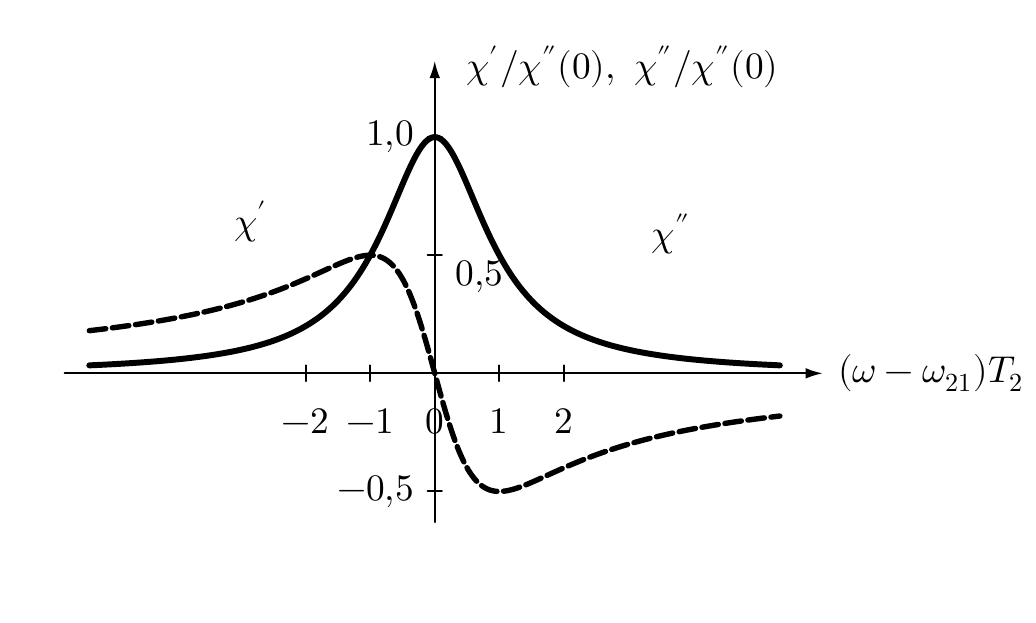
\begin{tikzpicture}[x=1cm,y=1cm,>=Latex,line cap=round,line join=round,font=\fontsize{15}{18}\selectfont]


% Authors' normalized dispersion and absorption on common detuning axis.
% χ''/χ''(0)=1/(1+δ²), χ'/χ''(0)=-δ/(1+δ²).
\path[use as bounding box] (0,0) rectangle (12.45,7.2);
\def\OX{5.17}\def\OY{2.81}\def\XX{.82}\def\YY{3.00}
\draw[axis] (.47,\OY)--(10.10,\OY);
\draw[axis] (\OX,.92)--(\OX,6.78);
\node[smalllabel,anchor=west] at (5.45,6.7) {$\chi'/\chi''(0),\ \chi''/\chi''(0)$};
\node[smalllabel,anchor=west] at (10.17,2.81) {$(\omega-\omega_{21})T_2$};
% Proper ticks on both axes; labels kept separate from the traces.
\foreach \t/\label in {-2/$-2$,-1/$-1$,1/$1$,2/$2$}{
  \draw[tick] ({\OX+\XX*\t},{\OY-.10})--({\OX+\XX*\t},{\OY+.10});
  \node[smalllabel,anchor=north] at ({\OX+\XX*\t},{\OY-.32}) {\label};
}
\foreach \t/\label in {-0.5/$-0{,}5$,1/$1{,}0$}{
  \draw[tick] ({\OX-.09},{\OY+\YY*\t})--({\OX+.09},{\OY+\YY*\t});
  \node[smalllabel,anchor=east] at ({\OX-.14},{\OY+\YY*\t}) {\label};
}
\draw[tick] ({\OX-.09},{\OY+\YY*.5})--({\OX+.09},{\OY+\YY*.5});
\node[smalllabel,anchor=west,fill=white,inner sep=1pt] at ({\OX+.22},{\OY+\YY*.5-.27}) {$0{,}5$};
\node[smalllabel,anchor=north] at (\OX,{\OY-.32}) {$0$};
\draw[curve,samples=460,domain=-5.35:5.35,smooth] plot ({\OX+\XX*\x},{\OY+\YY/(1+(\x)^2)});
\draw[curveb,samples=460,domain=-5.35:5.35,smooth] plot ({\OX+\XX*\x},{\OY-\YY*(\x)/(1+(\x)^2)});
% Callouts placed in non-intersecting white space, like the source.
\node[smalllabel,text=ScienceAux,anchor=west,fill=white,inner sep=2pt] at (2.55,4.74) {$\chi'$};
\node[smalllabel,text=ScienceCurve,anchor=west,fill=white,inner sep=2pt] at (7.85,4.58) {$\chi''$};

\end{tikzpicture}
\end{document}
